\documentclass{standalone}
\usepackage{tikz}
\usetikzlibrary{positioning,arrows.meta,shapes.misc,calc}

% COLORS
\usepackage{xcolor}
\colorlet{myred}{red!80!black}
\colorlet{myblue}{blue!80!black}
\colorlet{mybluee}{myblue!80!black}
\colorlet{mygreen}{green!60!black}
\colorlet{myorange}{orange!70!red!60!black}
\colorlet{mydarkred}{red!30!black}
\colorlet{mydarkblue}{blue!40!black}
\colorlet{mydarkgreen}{green!30!black}
\definecolor{mygray}{HTML}{D1D2D4}

\begin{document}
\begin{tikzpicture}[
    >=Stealth,
    block/.style={rectangle, rounded corners,  align=center},
]

% Placeholder image
\node[inner sep=0, outer sep=0] (image) at (0,0) {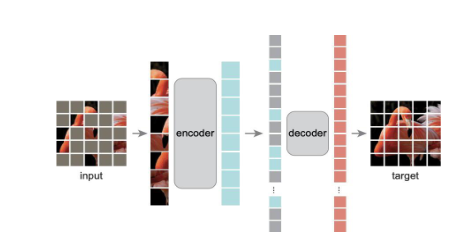
\includegraphics[width=15cm,height=8cm]{tikz/chapter11 - MAE.png}};
\node[fill=white, xshift=-4.6cm, yshift=-1.8cm] {Input};
\node[fill=white, xshift=5.6cm, yshift=-1.8cm] {Target};

\node[block,fill=mygray,xshift=-1.23cm, yshift=-0.45cm, minimum height=5cm,minimum width=1.5cm] (encoder) {\small Encoder};

\node[block, fill=mygray, right=2.1cm of encoder, minimum height=3cm, minimum width=1.5cm] (decoder) {\small Decoder};

\end{tikzpicture}

\end{document}